\chapter{Added Components}
In this chapter each component will be discussed with more detail, such as used technology and how does component map to docker containers
\section{SimBaD-Client}
From user perspective, the SimBaD-Client is the central point of the application. In this sec
The second section will talk about the two main application views- the configuration editor and the simulation pipeline view. Finally, the way of serving application will be discussed and what will be placed in docker container responsible for SimBaD-Client.
\subsection{Technology}
\subsubsection{Overview of frameworks}
The web development ecosystem in current year is as rich as it is complicated.  For anything other than a simple static website, many tools are necessary to solve problems such as making the website work in different browsers, internationalization, or production and development builds. There are numerous frontend JavaScript frameworks, such as Angular, React or Vue to name a few. One can achieve exactly the same result using those frameworks, so the choice between mainly comes down to developer preference. For the SimBaD-Client, Angular is the framework of choice, due to its excellent support for Typescript, tooling with Angular-CLI, great UI library - Angular Material and OpenApi Codegen support, used to generate client libraries communicating with SimBaD-Pipeline-Server API. 
\subsubsection{Monorepo pattern}
The project was bootstrapped with Angular-CLI and NX using monorepo pattern. Monorepo, is a pattern that helps organize and share code between multiple JavaScript applications. Code in monorepo, as the name indicates is put in single repository. Monorepo ensures that everything at a single commit works together - for code in separate repositories, the state of application is a combination of several commits from each repository. Another benefit, especially important for frontend applications, is that it allows to centralize the build system and and tool chain - all of the code in monorepo is build using Angular-CLI and depends on same libraries. It makes easy to split the code into libraries, and to compose applications using those libraries. For SimBaD-Client it allows to split the client code into apps, such as SimBaD-Client app, developer server for building frontend independently from backend, and shared API and UI libraries. The CI process is also simplified, as each change and applications and libraries that are affected by this change can be tested, and pass for such tests proves that each application in monorepo works as indented.
\subsubsection{Reactive programming and store architecture}
Reactive programming is a programming paradigm that deals with asynchronous data streams - sequences of some kind of events ordered in time. Data streams can be created from anything, from click events, http calls to user inputs or variable declarations. Streams can be then manipulated, for example they can be filtered, merged, mapped to other streams. Those streams can also be "subscribed to" or "consumed" to produce some kind of side effect, like showing notification in UI, when some API returns specific status. Reactive programming changes the way that application components communicate with each other. Instead of pushing data directly into components, or components asking explicitly for data, in reactive programming they automatically "react" to data changes. The most popular library for Reactive programming is Rx (Reactive extensions), and RxJS is the JavaScript version of this library. For web applications, when almost all code, including simple console.log() statements is executed asynchronously, and there is multitude of UI or data related Events to react to, RxJS allows to write code that handles those events in a clean, maintainable and concise way.
\begin{figure}[h!]
	\centering
		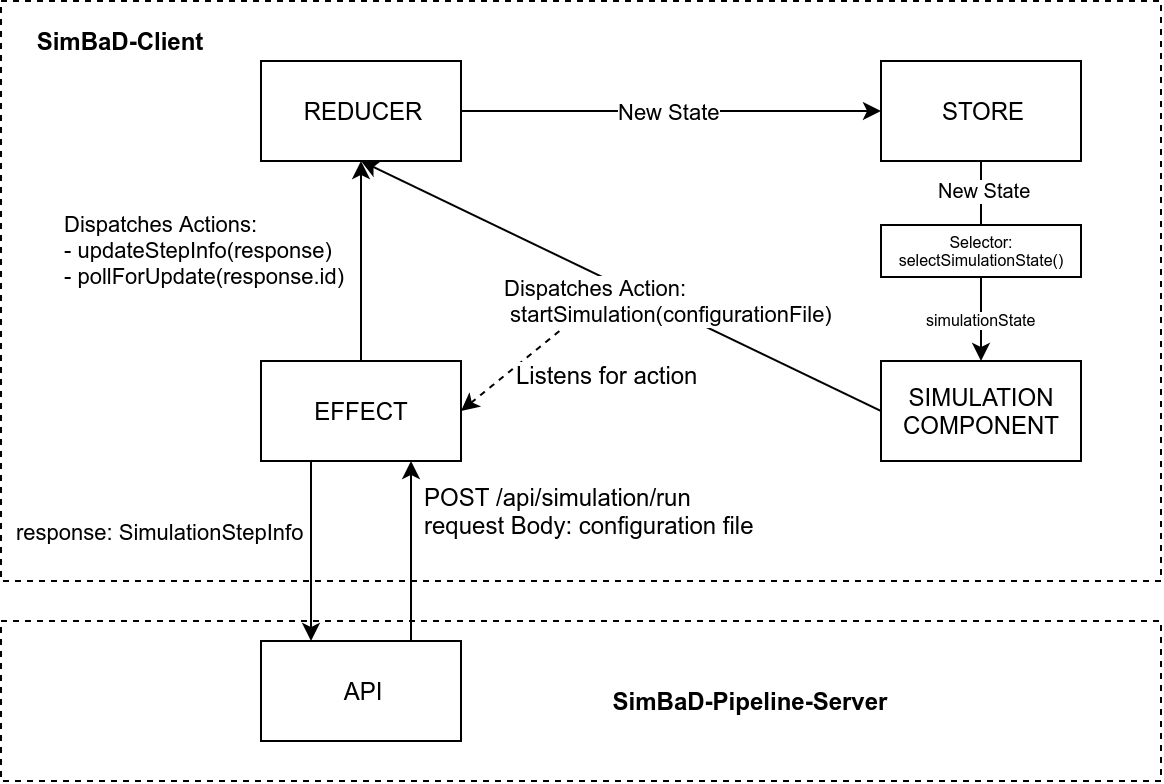
\includegraphics[width=0.9\linewidth]{diagrams/ngrx.png}
	\caption{Example of NgRX flow in SimBad-Client}
	\label{fig:ngrx}
\end{figure}
Reactive programming works very well with store architecture. The store can be thought of as a client-side database, where all data needed by application resides. The store reflects the complete state of application.
NgRX uses the RxJS library heavily - the store itself is an obervable, an components need to subscribe to the store observables to get the data. Store architecture solves problem of passing data between components.
In angular, data can be passed between components in server ways - from parent to child using Input() member variables, from child to parent using EventEmmiters() and between unrelated components using services. Problems arise when data needs to be passed several levels down in component tree - the root component has the data, and the leaf components needs this data, however for the component nodes along the way, that do not need the data, extraneous Input properties must be added. Store architecture bypasses that problem, by providing single source of truth or the store for all of the components to get data from and push data to. When actor such as user or server changes some data, this change is pushed to store, and automatically reflected in all of the components. NgRX is a library that provides tools to add store architecture to application. 
NgRx consists of several building blocks - actions, reducers, effects and selectors. The components can alter state of application or by dispatching actions to store. Actions consists of type - unique action identifier and payload - the data that is needed to change the state. Reducer is a pure function that accepts two arguments - current state of application and action. Reducer analyzes the action and returns new state that is a combination of previous state and action payload. Side effect can be something like making a http call, or showing a notification. The effects trigger when specific action is dispatched to store, and can be used to trigger side-effect based on those actions. Effects can also dispatch another action to the store, for example they can push response received from http call. Single effect can be triggered by multiple action, can dispatch multiple actions and single action can trigger multiple effects. The store can be pretty big object, and components need only a part of it. Selectors facilitate this by allowing the components to get or in other words "select" only parts of the store. In the figure \ref{fig:ngrx}, example NgRX flow trigerred by user starting the simulation is shown.

The user action, for example clicking a button, causes the component responsible for simulation view to dispatch startSimulation() action with simulation configuration file as its payload. This triggers two separate NgRX flows. In the first one, the action is passed to the reducer, and new state with added information that simulation has started is generated. Then the store observable emits new data and component receives a slice of this data, based on selector. The second flow starts with effect, that reacts to startSimulation Action being triggered. This effect makes then POST request to Simulation-Pipeline-Server to start simulation, and receives the information about the first simulation step - the SimBaD-CLI step. Effect then dispatches two actions with, response as a payload, one to update step info in store, and one to start polling for step info changes. Those actions then are handled by reducer, new store state is emitted and passed to component. If dispatched actions trigger any effects, another flow starts.
\subsection{Configuration editor view}
To start simulation process user needs to pass simulation configuration file or SCF. This file has tree-like structure and contains various objects and parameters that control the simulation process. Although those objects need have predefined value types, ranges, or enums, the exact definitions did not exists, and had to be created. Detailed description of this file and how to add new parameters to simulation can be found in appendix \ref{appendix:A}.
\begin{figure}[h!]
	\centering
		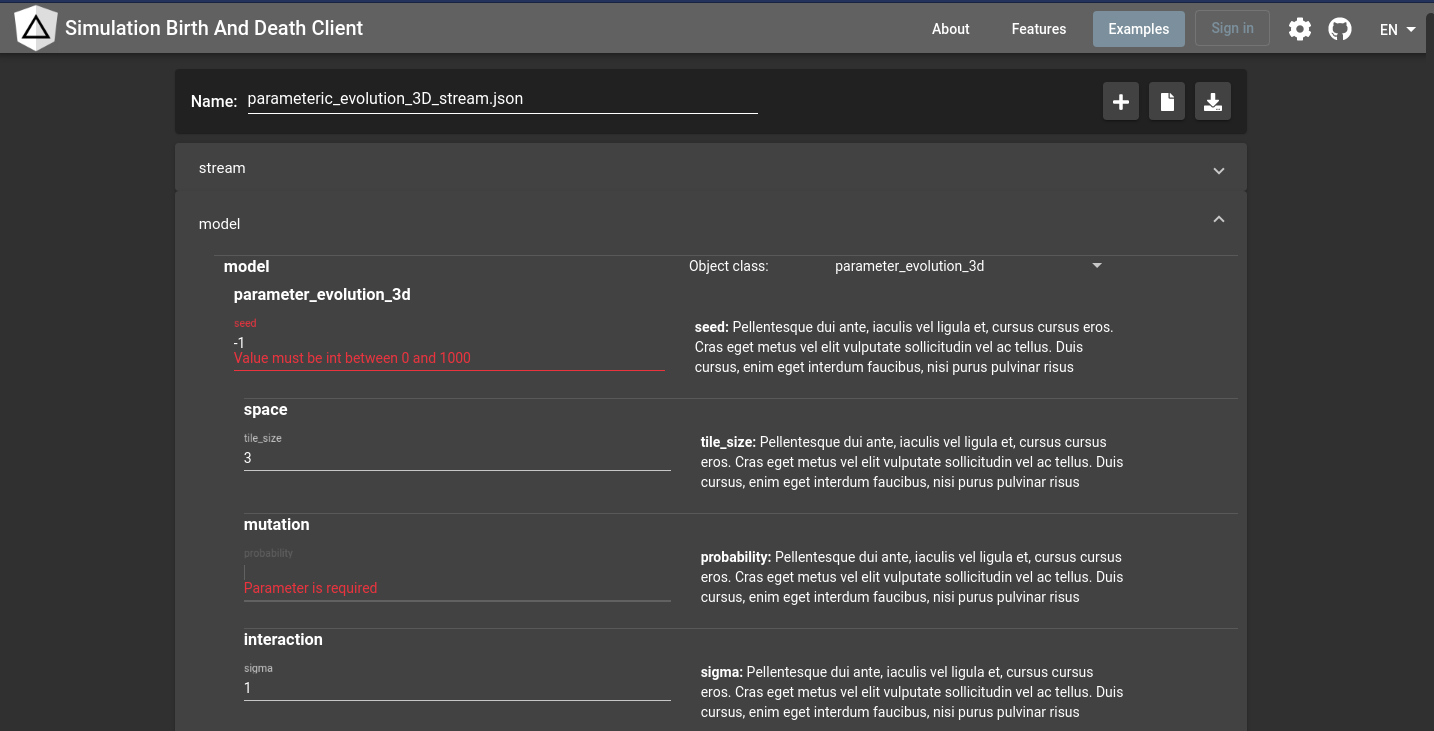
\includegraphics[width=0.9\linewidth]{screens/conf-view.png}
	\caption{The configuration editor view}
	\label{fig:conf-view}
\end{figure}
To enable user to generate valid configuration, configuration editor was created. Configuration editor generates forms that validate the parameter values entered by user against their definitions. The form has tree structure that maps to configuration. Additionally, each form input associated with parameter displays validation messages, and parameter description. The form is generated dynamically, and adding or changing definition in object definition does not break the form, though it requires to rebuild application. The user can create new configuration, and download and upload the configuration from .json file.  The SimBaD-CLI supports two file formats: .json and .simbad which is an alias to default boost:tree format. As the changes in configuration are dispatched to store, the configuration can be shared between different components. 
\begin{figure}[h!]
	\centering
		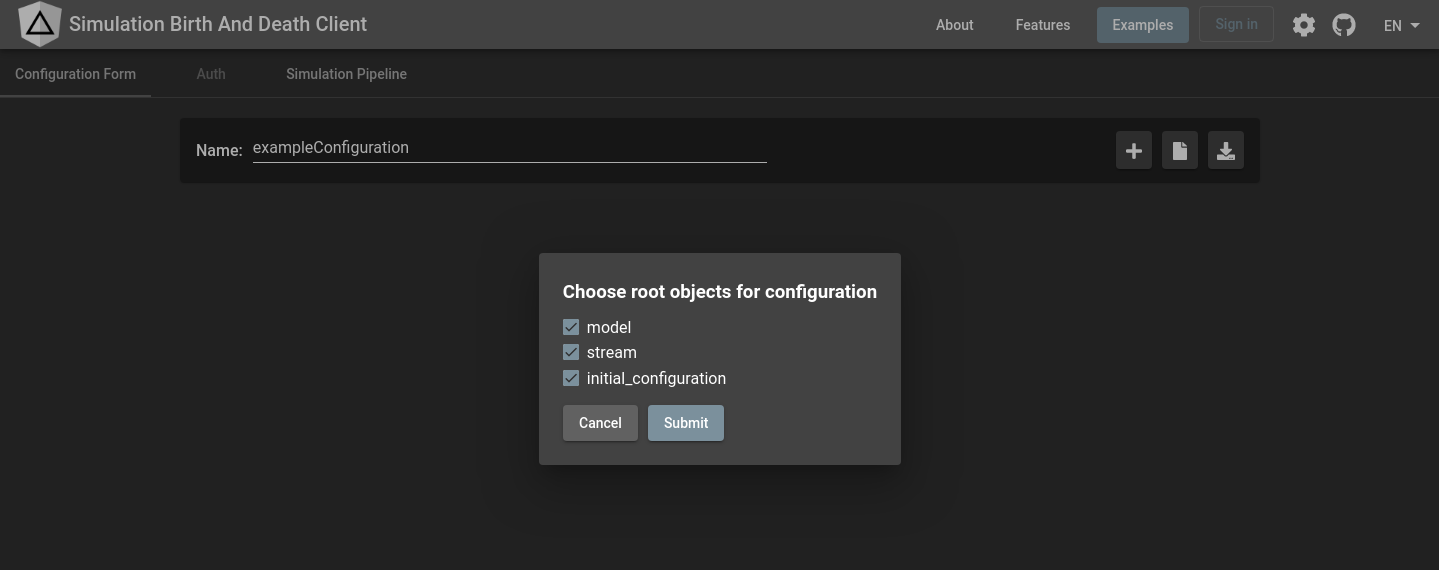
\includegraphics[width=0.9\linewidth]{screens/configuration-view-modal.png}
	\caption{Creating new configuration}
	\label{fig:conf-view-new}
\end{figure}
\subsection{Simulation pipeline view}
The second view of the application is the view that allows to monitor the simulation process. User can start simulation pipeline using this view. To start it, user can upload configuration file, or when present in store, use the previously edited configuration file. Additionally, user is able to load the results of last simulation. Each major change in step such as finishing or starting a step is accompanied by proper notification.
The simulation pipeline view consists of 3 main components, each responsible for different simulation step. Each of those components allows to view the current simulation status with information such as current step runtime status, the context of a step, and when step finishes, the resulting output files (also called simulation artifacts). Each artifact can be downloaded in .zip form, and for images, it can also be displayed. For the SimBaD-CLI view, visible in the figure \ref{fig:sp-cli}, additional metrics regarding the process executing the simulation are displayed - the CPU usage and ram usage. 
\begin{figure}[h!]
	\centering
		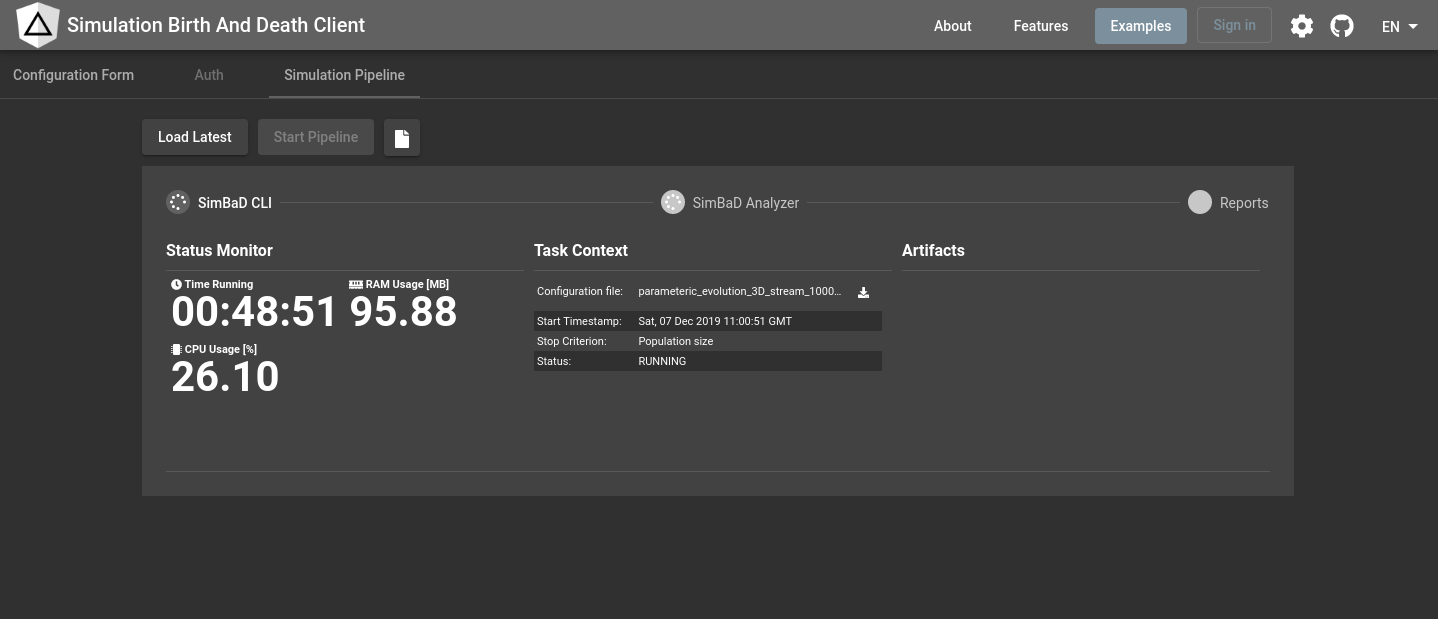
\includegraphics[width=0.9\linewidth]{screens/cli-view.png}
	\caption{Simulation pipeline view: CLI step}
	\label{fig:sp-cli}
\end{figure}
For the analyzer-view, there's a link to the Spark UI dashboard and progress bar that displays information about total progress of analyzer job, based on already created artifacts. This view can be seen on the figure \ref{fig:sp-analyzer}.
\begin{figure}[h!]
	\centering
		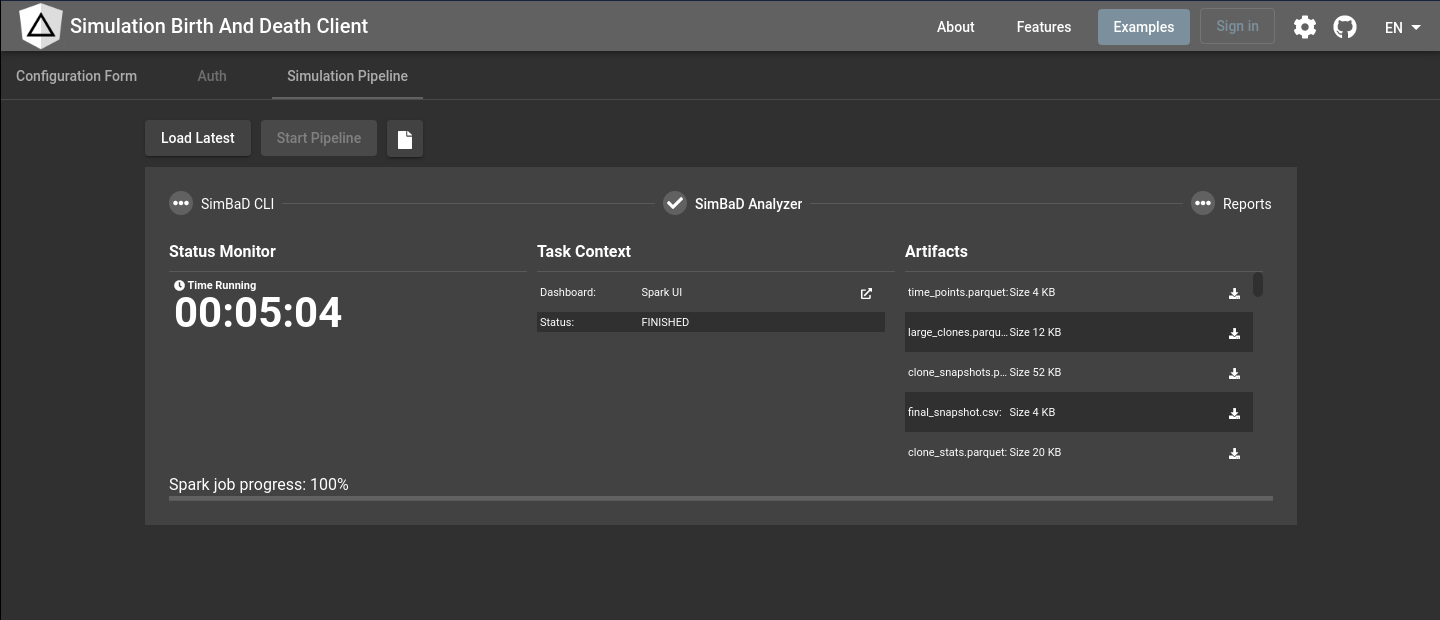
\includegraphics[width=0.9\linewidth]{screens/analyzer-view.png}
	\caption{Simulation pipeline view: Analyzer step}
	\label{fig:sp-analyzer}
\end{figure}
Finally the last step of this view is the report step. Apart from option to download the resulting plots, the user has also option to display the plots in browser. Example display of such plot is shown on the figure \ref{fig:sp-report-muller}.
\begin{figure}[h!]
	\centering
		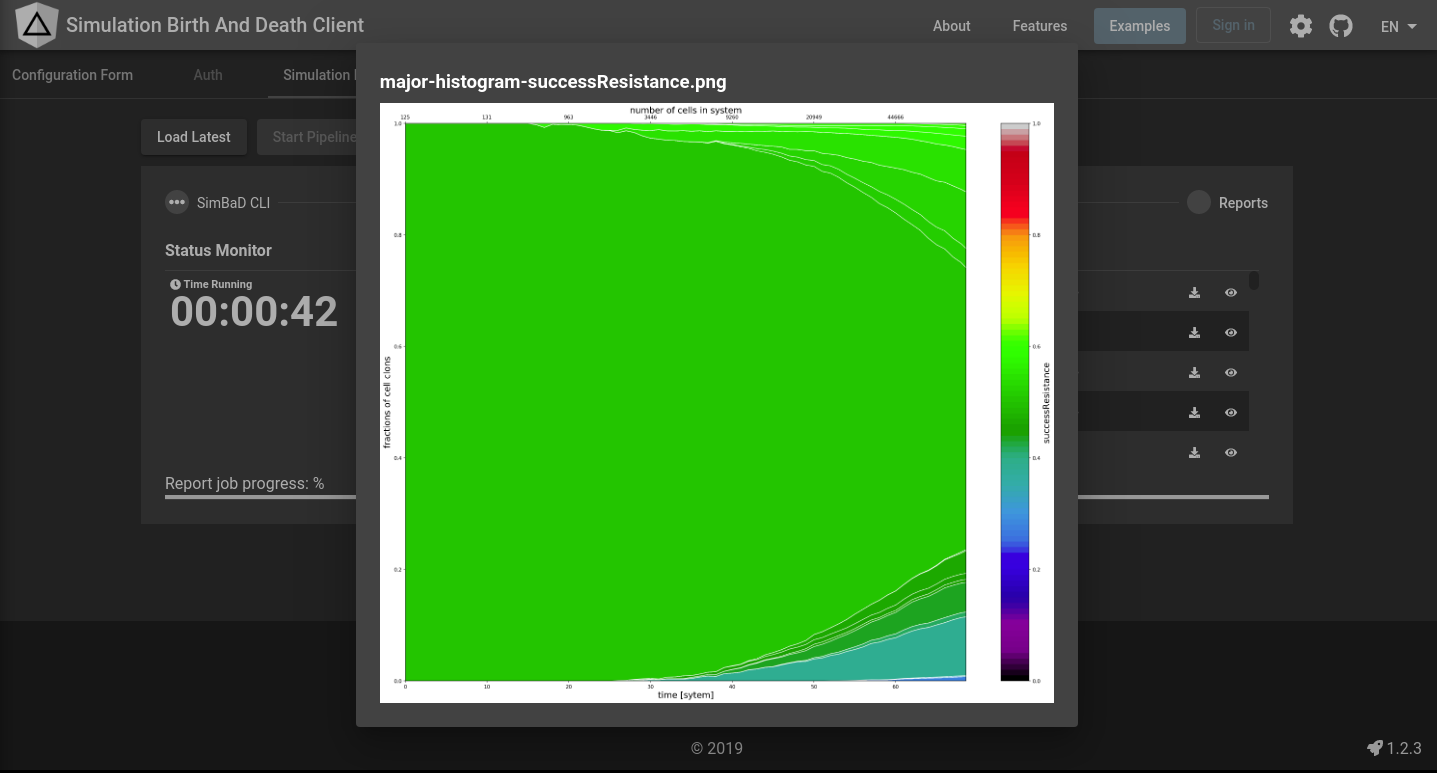
\includegraphics[width=0.9\linewidth]{screens/report-view-muller.png}
	\caption{Report view: mullerplot}
	\label{fig:sp-report-muller}
\end{figure}
\newpage
\subsection{Serving the client}
To server application from docker contaienr first it is necessary to build it. The application can be build in two ways- the development build and the production build. The development build contains non minified code with sourcemaps that is suitable for debugging.  Minification is a process of removing redundant data from the code (such as whitespace, comments or verbose function and variable names). and sourcemaps are files that map compressed and transpiled javascript code to its original source files. Such build should not be server to the user, as it not optimized in size, and contains informations valuable only to developer. The production on the other hand, reduces the size of the bundle applying minification tree shaking and ohter techinques. Such build is suitable to be actuall served to user but needs an actual server to host it. There are many http servers, but for the purpose of this application the nginx was used. Apart from serving the files, the nginx also is used as reverse proxy to SimbAd-Pipeline-Server. 
There are two steps to create docker image for this component. First, all of the npm packages necesary to build the application must be installed, and after building it, the resulting files must be copied to the /usr/share/nginx folder. To avoid increasing the image size the docker multi-stage builds feature was used. The dockerfiles for this component is visible on listing.
\begin{lstlisting}[label=list:sc-docker,caption=Dockerfile used to build SimBaD-Client, basicstyle=\footnotesize\ttfamily]
FROM node:11.1.0 as npm_builder
COPY ./package.json /usr/simbad-client/app/package.json
COPY ./package-lock.json /usr/src/app/package-lock.json

WORKDIR /usr/simbad-client/app
RUN npm install --silent

FROM npm_builder as builder
COPY . /app
ENV PATH /app/node_modules/.bin:$PATH
WORKDIR /app
RUN npm run build

FROM nginx
COPY --from=builder /app/dist/projects/simbad-client /usr/share/nginx/html
\end{lstlisting}
Dockerfile is split into three stages, the first npm\_builder extends the community image with installed NPM and node.
The package.json files containing client dependencies are copied onto the file and the packages from this file are installed. The second stage is builder, used to generate production build. The last stage is Nginx. It starts with nginx image from Dockerhub, to which the resulting build files are copied. The size of resulting image is the size of Nginx image + the size of build output - it does not have all of the node toolchains or node modules installed, and that saves over 1GB of disk space.
\section{SimBaD-Pipeline-Server}
This component is at the center of the simulation. It receives commands from the client and manages whole simulation process.
As discussed in chapter \ref{chapter:arch}, the SimBaD-Pipeline-Server must communicate with client using HTTP RPC API, store data in shared volume and sqlite database, and be able to communicate with existing components placed in same container, by executing the scripts and binaries directly, or with component in separate container, using HTTP RPC API and SSH. In the following sections the technology choices and inner mechanisms of working wil be discussed.
\subsection{Technology}
\subsubsection{Choice of framework}
Almost any programming language has some framework dealing with writing http servers. In that regard, the choice of the framework mainly depends on developer preference, as the http capabilities of the component can be created using any of those frameworks. The important factor is how well will the language work with existing binaries and scripts. As the server needs to be able to call python scripts and C++ binaries the choice narrows down to python web frameworks. Two most popular ones are Flask and Django. Out of those two, flask was chosen, mostly due to the fact that it gives developer much more freedom than Django, and allows to tailor application to specific use case, without imposing standard model, as Django. Django comes with extensive toolkit for serving HTML and server-side rendering, which is not needed for the SimBaD-Pipeline-Server, because it is used as web service, the actual serving of SimBad-Client is delegated to Nginx.
The flask is extendable but that also means that it needs to be manually extend to fit the needs, and the features like splitting the api routes into separate files or setting up ORM need to be done manually.
\subsubsection{ORM}
To save information about simulation ORM was used with help of SQLAlchemy. Overall simulation information was divided into several objects. Each simulation step generates output files, such files are represented by the Artifact object. This object has information about the path to actual file in the shared filesystem, which simulation and which simulation and which step generated the artifact, its size and timestamp when it was created. Individual simulation steps are represented by SimulationStep object. This object has information about current state and runtime info, resulting artifacts, and timestamps associated with step. Definition of SQLAlchemy model can be seen on listing.
\begin{lstlisting}[label=list:sp-sqlalchemy,caption=SimulationStep SQLAlchemy model, basicstyle=\footnotesize\ttfamily]
class SimulationStep(Base):
    __tablename__ = 'steps'
    RELATIONSHIPS_TO_DICT = True

    id = Column(Integer, primary_key=True)
    simulation_id = Column(Integer, ForeignKey('simulations.id'))
    started_utc = Column(DateTime)
    finished_utc = Column(DateTime)
    origin = Column(String())
    celery_id = Column(String())
  
    cli_runtime_info = relationship(
        "CliRuntimeInfo", 
        uselist=False, 
        backref="steps"
    )
  
    analyzer_runtime_info = relationship(
        "AnalyzerRuntimeInfo", 
        uselist=False,
        backref="steps"
    )
  
    artifacts = relationship("Artifact", backref="steps")
    
    def __json__(self):
        return ['id', 'simulation_id', 'started_utc', 'finished_utc',
                'origin', 'artifacts', 'cli_runtime_info',
                'analyzer_runtime_info']
\end{lstlisting}
SimualtionStep model extends the Base SQLAlchemy class which enables access to SQLAlchemy functionality, such declaring tables, primary keys or relationships between object. The \_\_json\_\_ method is used, when model is serialized to json, for example, for status responses to client. The list it returns defines which properties will be in serialized object. 
\subsubsection{Task queue}
Waiting for simulation to finish, before returning some sort of response to the client is not feasible, as the simulation process takes a lot of time, the http request should not be open for that long, and the user is deprived of simulation progress updates. To solve that, after receiving the server should start running the simulation in background, and return confirmation that simulation is started, along with other information that enables the client to poll for status changes.
Though only one simulation process should be run at a given time, multiple simulations should be able to be scheduled by multiple clients for later execution, and that calls for simulation task queue. To enable that functionality, Celery framework was used. Celery allows to schedule and execute tasks in synchronous and asynchronous way. At the start of the server, it searches for tasks in code(annotated by @celery.task), and starts worker threads that will execute those tasks.
To queue task, celery needs a way to transport messages, also called a messagge broker. The two main choices for brokers are RabbitMq and Redis. As Celery has support for each of those brokers, the primary factor was the size of docker image, and as the size of official Redis image is slightly smaller, Redis was chosen.
Celery allows to compose primitive celery tasks into different ways, to change the order of execution. Tasks in celery chains are executed in sequence, and the output of previous task is passed as first argument of current task, which is a perfect solution of simulation pipeline. Example of such chain is shown on listing \ref{list:sp-celery-chain}. 
\begin{lstlisting}[label=list:sp-celery-chain,caption=Celery chain - Main Simulation task, basicstyle=\footnotesize\ttfamily]
@celery.task(name='SIMBAD-SIMULATION-MAIN')
def run_simulation(artifact_id) -> AsyncResult:
    result = chain(
        cli_step.s(artifact_id),
        analyzer_step.s(),
        reports_step.s()
    ).apply_async()
    return result
\end{lstlisting}
The celery group allows to execute task in parallel, which is useful in the report step, as each report script can be executed independently. Celery groups, however cannot be chained together, so for plots the main primitive that was uses was chord. Chord is a task that is executed after all of the task in groups are executed. Example of chord is shown on the listing \ref{list:sp-celery-chord}. The chordfinisher task on the listing is a dummy tasks, and its used as a workaround for inability to chain groups.
\begin{lstlisting}[label=list:sp-celery-chord,caption=Start simulation endpoint, basicstyle=\footnotesize\ttfamily]
@celery.task(bind=True, name='SIMBAD-MAJOR-CLONES-MULLERPLOT-STATS')
def major_clones_mullerplot(self, workdir: str):
    param_names = [
        'birthEfficiency',
        'birthResistance',
        'lifespanEfficiency',
        'lifespanResistance',
        'successEfficiency',
        'successResistance',
    ]

    tasks = []
    for name in param_names:
        tasks.append(major_clones_mullerplot_histogram.s(workdir, name))
    chord(tasks, chordfinisher.si()).apply_async()
    return workdir
\end{lstlisting}
Example of combining Flask endpoitns, ORM and Celery task together is shown on listing \ref{list:sp-api-run}. The endpoint shown, is the endpoint that starts the simulation process.
First, the configuration file is extracted from request body, and setup for new simulation process is started. The result of setup is Artifact representing the simulation configuration file. Id of object representing SimBaD-CLI step is extracted from artifact and passed to simulation task. The simulation task is started and background, changes to database are commited, CLI step object is serialized to json and returned as response to SimBaD-Client.
\begin{lstlisting}[label=list:sp-api-run,caption=Start simulation endpoint, basicstyle=\footnotesize\ttfamily, language=python]
@simulation_api.route('/start', methods=['POST'])
def start():
    request_data: dict = request_to_json(request)
    conf: Artifact = setup_workdir(request_data)
    db_session.begin()
    db_session.flush()
    step = db_session.query(SimulationStep).get(conf.step_id)
    task = run_simulation.delay(conf.id)
    step.celery_id = task.id
    db_session.commit()
    return jsonify(step)
\end{lstlisting}
\subsection{Task executors}
For different configurations, different components of simulation pipeline can be placed on different docker containers or even on different machines. To enable easy switch between ways of executing certain task, the task executor interface was proposed. 
\begin{lstlisting}[label=list:sp-ex-base,caption=Base executor, basicstyle=\footnotesize\ttfamily, language=python]
class BaseExecutor:
    def __init__(self):
        self.is_finished = False
        self.result = None
        self.status = None

    def execute(self, in_file: Artifact) -> None:
        pass

    def cleanup(self) -> None:
        pass
\end{lstlisting}
This interface has to be implemented for each object managing simulation step. The main three implementations of this interface are LocalExecutor, HttpExecutor and SSH Executor. Use of task executors in celery tasks split the responsibilities - celery task acts as a client that starts task and periodically asks for updates or results, and the task executor act as a server, that actually executes the task. Because the celery task does not actually executes the task but rather uses an interface, the way which task are executed can be easily change. The interface is consistent for executors that run binaries and scripts locally and executors that make http calls to another server to start a task.
For the purpose of demonstrating such concept, each of those executors was implemented for a simulation step - LocalExecutor for SimBaD-CLI, HttpExecutor and SshExecutor for SimBaD-Analyzer step. The fragment of local executor implementation is shown on the listing \ref{list:sp-exec-local} and how executor is used from celery is shown on listing \ref{list:sp-exec-local-use}.
\begin{lstlisting}[label=list:sp-exec-local,caption=Fragment of LocalExecutor for SimBaD-CLI, basicstyle=\footnotesize\ttfamily, language=python]
def execute(self, in_file: Artifact) -> None:
    thread = threading.Thread(target=self.run_cli, args=[in_file])
    thread.daemon = True
    thread.start()
    return
    
def run_cli(self, conf: Artifact) -> None:
    self.status.step_id = conf.step_id
    out_path = '{}/cli_out.csv'.format(conf.get_workdir())
    conf_path = conf.path

    with open(out_path, 'w') as f:
        process = subprocess.Popen(
            (self.executable_path, conf_path), 
            stdout=subprocess.PIPE
        )
        process_info = psutil.Process(process.pid)
        counter = 0
        for c in iter(lambda: process.stdout.read(1), b''):
            counter += 1

            if counter % 1000000 == 0:
                memory = process_info.memory_info().rss / 1000000
                cpu = process_info.cpu_percent()
                self.status.memory = memory
                self.status.cpu = cpu
                # TODO: parse some additional status data from stderr?

            line = c.decode('utf-8')
            f.write(line)
\end{lstlisting}
As long as the specific executor is implemented for task, it can be used. Which executor is used to which task, as well as other configuration options can be set using docker .env files, wich will be described more in section \ref{sec:dockerconf}.
\begin{lstlisting}[label=list:sp-exec-local-use,caption=Use of LocalExecutor for SimBaD-CLI step, basicstyle=\footnotesize\ttfamily, language=python]
@celery.task(bind=True, name='SIMBAD-CLI')
def cli_step(self, artifact_id: int) -> int:
    conf: Artifact = db_session.query(Artifact).get(artifact_id)
    ...
    executor: BaseExecutor = get_cli_executor()
    executor.execute(conf)

    while executor.is_finished is not True:
        db_session.begin()
        runtime_info.cpu = executor.status.cpu
        runtime_info.memory = executor.status.memory
        db_session.commit()
        sleep(POLLING_PERIOD)

    result: Artifact = executor.result
    ...
    return result.id
\end{lstlisting}
The SSH Executor is functionally identicall to HTTP Executor, the only difference that before the first connection, it opens SSH tunnel to remote server, using the SSHTunnelForwarder from sshtunnel python library. 
\section{SimBaD-Analyzer-Server}
Extracting component to separate docker container requires adding http layer on top of it, which will be used by the aforementioned Http and SSH TaskExecutors on the pipeline server. In the proposed system, this such layer, named SimBaD-Analyer-Server was added on top of the SimBaD-Analyzer component. 
\subsection{Technology}
To maintain consistency across apps, and other reasons stated in frameworks overview in section, Flask was selected as a framework of choice for managing http api. The API definitions, as it was the case server-client communication, were defined using OpenAPI. Python and Flask dependencies were added tp existing docker image containing spark ecosystem and built Simbad-Analyzer jars. Propsed architecture assumes that all of the components have access to the same shared volume, to make that possible for containers on separete hosts, sshfs docker extension was added. This extensions allows to create shared docker volume, and allow acces to it through ssh connection.
\subsection{Integration with Spark}
In its structure, the extension to analyzer is very similar to TaskExecutor. Properties and methods of task executor are now mapped to endpoints - the execute method is now the /api/analyzer/start endpoint, the result property is now a /api/analyzer/result endpoint and so on. Making a POST request to /api/analyzer/start endpoint, with path to the output file of SimBaD-CLI, starts the step. Before submitting the job to spark, checkpoints and spark warehouse that might have been created by previous simulation run need to be cleared.
\begin{lstlisting}[label=list:sp-exec-local-use,caption=Use of LocalExecutor for SimBaD-CLI step, basicstyle=\footnotesize\ttfamily, language=python, numbers=left]
@app.route('/api/analyzer/start', methods=['POST'])
def start():
    global analyzer_status
    if analyzer_status['status'] is 'BUSY':
        return {"status": "failed"}, 402
        
    request_data: dict = request_to_json(request)
    path: str = request_data['path']
    analyzer_status['status'] = 'BUSY'
    start_analyzer(path)
    return "OK", 202
\end{lstlisting}
Submitting tasks to spark is done through running shell commands. Two commands must be run, first to read the generated by the CLI and second to analyze it. Method executing this command can be seen on listing. After submitting the Analyzer job to spark, daemon starts in background that periodically updates the progress of simulation, by checking how many of the required files files were created. If all of the required files were created, the global result variable is set to list of paths of created files, and can be retrived by TaskExecutor running on SPS through /api/analyzer/result endpoint.
\begin{lstlisting}[label=list:sp-exec-local-use,caption=Use of LocalExecutor for SimBaD-CLI step, basicstyle=\footnotesize\ttfamily, language=python, numbers=left]
def start_analyzer(path: str) -> None:
    ...
     reader_cmd = "spark-submit" \
                  " --master local " \
                  "--class analyzer.StreamReader " \
                  "/jar/analyzer.jar {} {}"\
                  .format(path, stream_dir)
    reader_process = subprocess.Popen(reader_cmd, shell=True)
    reader_process.wait()
    analyzer_cmd = "spark-submit" \
                   " --master local " \
                   "--class analyzer.Analyzer /jar/analyzer.jar {} {}"\
                   .format(stream_dir, spark_out_dir)
    subprocess.Popen(analyzer_cmd, shell=True)
    thread = threading.Thread(target=update_runtime_info)
    thread.daemon = True
    thread.start()
    return
\end{lstlisting}
\section{Docker containers for components}
The first container that needs to be added is the contaienr with nginx that hosts the SimBaD-Client code. The Simbad-Pipeline-Server component requires three docker containers to run. First container serves the http api that is used by the client. Second container runs the Celery worker, that executes scheduled task. Those two containers share the same image. The third component is a Redis image, that acts as a message broker for Celery. The last container is a container for simbad-analyzer-server, containing the HTTP API extension and SimBaD-Analyzer. The diagram visualizing all of the containers can bee seen on the figure \ref{fig:docker-containers}.
\begin{figure}[h!]
	\centering
		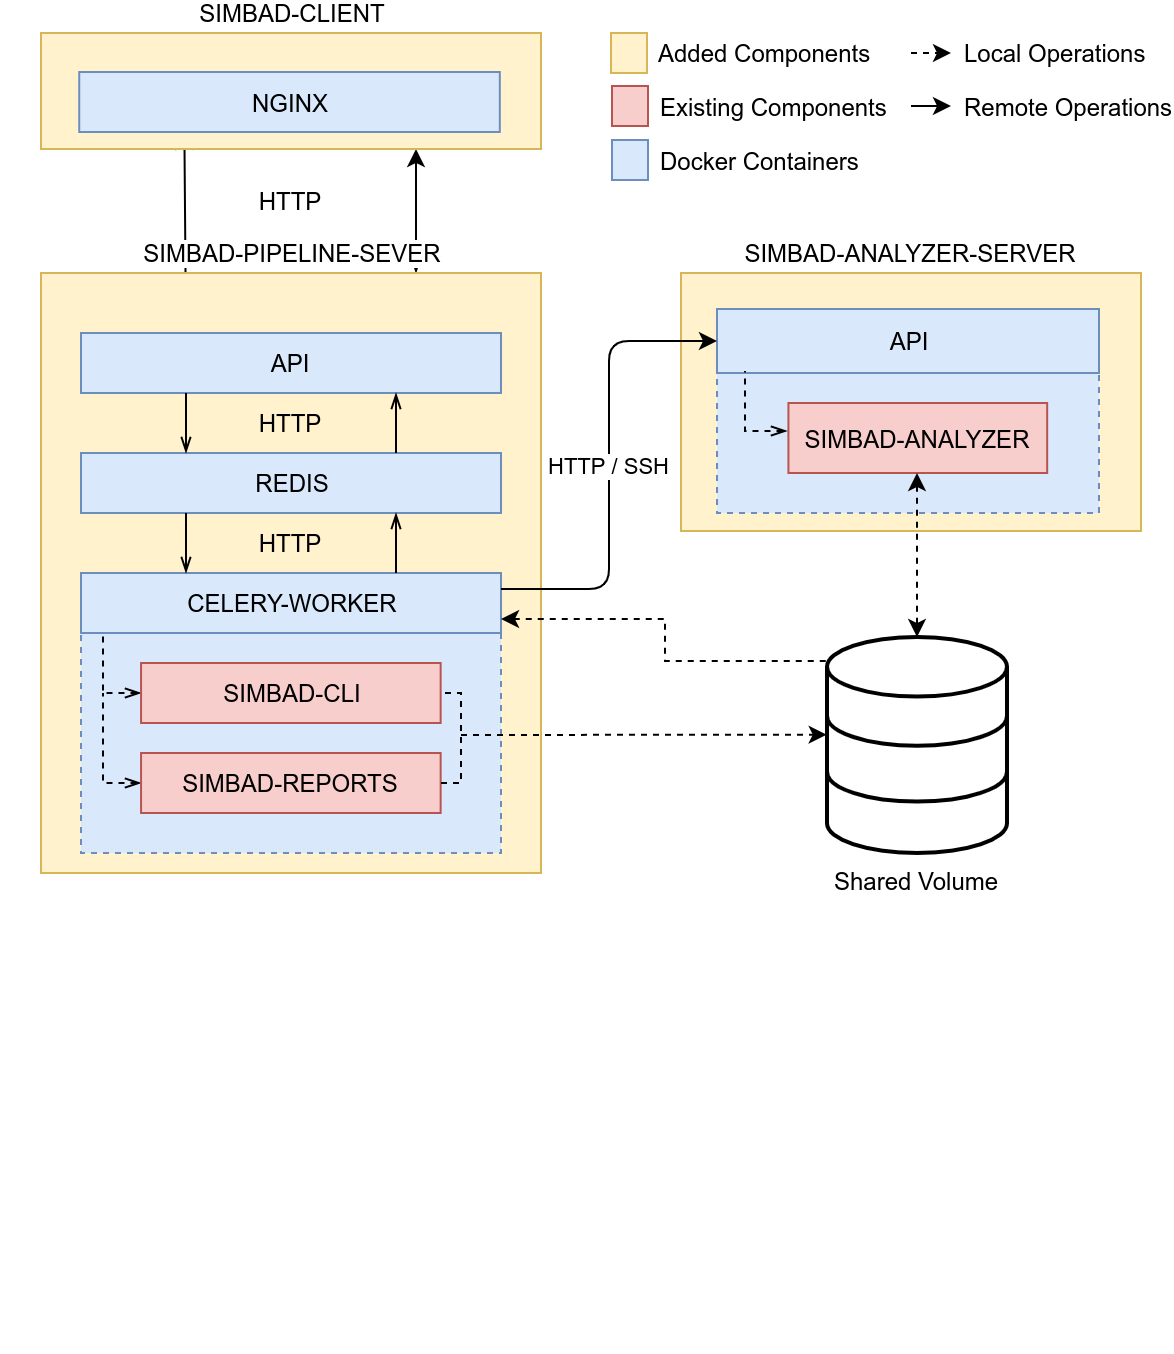
\includegraphics[width=0.9\linewidth]{diagrams/docker.png}
	\caption{Diagram of docker-compose containers}
	\label{fig:docker-containers}
\end{figure}
When simulation systems grows in a decoupled way, the number of docker container to manage also grows. To aid managing these containers, docker-compose was used. This tool can be used to define and manage application consisting of several components, placed on separate docker containers. The definition of application is placed in single docker-compose.yaml file. One can define services, shared volumes and networks in this file, and the start whole application using single commands. Contaienrs are build from images that can be defined using Dockerfiles or downloaded from DockerHub. Additionally, the network and volume definitions also can be placed in this file. Developing such system causes a need for two separate docker-compose files, one for the developer, that builds docker images from source, and one for user, so called, that pulls prebuild images from DockerHub. The docker-compose file that defines all of the simulation components using prebuild images is depicted on listing.  \ref{list:docker-compose}. 
\begin{lstlisting}[label=list:docker-compose,caption=prod-docker-compose.yaml file, basicstyle=\footnotesize\ttfamily, numbers=left, escapechar=|]
version: '3.4'
services:
  client:
    image: jsokolowski/simbad-client
    container_name: simbad-client
    ports:
      - "8080:80"
    volumes:
      - ./nginx.conf:/etc/nginx/nginx.conf
  pipeline:
    image: jsokolowski/simbad-pipeline-server |\label{line:sp}|
    container_name: simbad-pipeline-server
    command: python entrypoint_api.py --port 8081 --debug
    env_file:
      - ./docker.env
    ports:
      - "8081:8081"
    volumes:
      - ../data:/usr/data
  worker:
    image: jsokolowski/simbad-pipeline-worker
    container_name: celery-worker
    links:
      - analyzer-server
    command: celery worker -A entrypoint_celery.celery --loglevel=info
    env_file:
      - ./docker.env
    volumes:
      - ../data:/usr/data
  analyzer-server:
    image: jsokolowski/simbad-analyzer-server
    container_name: simbad-analyzer-server
    command: python3 app.py --port 5000 --debug
    env_file:
      - ./docker.env
    volumes:
      - ../data:/usr/data
      - ./log4j.properties:/opt/spark-2.4.3-bin-hadoop2.7/conf/log4j.properties
    ports:
      - "5000:5000"
      - "4040:4040"
  redis:
    image: redis:alpine
    container_name: redis
    ports:
      - "6379:6379"
\end{lstlisting}
All of the simulation component containers are defined under the "services" tag, for example, analyzer-server tag defines configuration of SimBaD-Analyzer-Server component. The image key, under the analyzer-server, specifies from where to pull the prebuild image. The "command" key specifies what command needs to be executed after container is started. The env\_file key specified the path to file with environmental variables, that need to be set inside of container OS. This file is also primary method of configurating the system and will be described in more detail in section  \ref{sec:configuration}. Shared volumes and files that need to be placed inside container can be defined using the volmes key. First entry under that key is a shared volume, where the simulation files will reside. The " ../data:/usr/data" syntax, means that the local data folder will be mounted as /usr/data folder inside of the container. The "value:value" syntax in general can be interpreted as "HOST:CONTAINER". Similiary, second entry under this key copies local configuration file for log4j, that is used to configure logging in spark. The last key is ports which is used to define which ports need to be exposed in container. The syntax "5000:5000" means that the through port 5000 on docker host, it is possible to access port 5000 on docker container. Port 5000 on this container exposes the  Simbad-Analyzer-Server API and port 4000 is used to access SparkUI dashboard.
\section{System Configuration}
Two main sources of configuration are the docker-compose files and .env files. Form the compose files it is possible to specify ports and paths to data. The .env file contains the definition of environment variables that will be set in , that every containerfile is apa 
\subsection{Default configuration}
\label{sec:configuration}